% Компіляція: lualatex -shell-escape main.tex
\documentclass[12pt,a4paper]{article}
\usepackage{fontspec,polyglossia}\setdefaultlanguage{ukrainian}\setmainfont{NewComputerModern10}\setmonofont{Noto Sans Mono}[Scale=.82]
\usepackage{amsmath,booktabs,caption,enumitem,float,fvextra,geometry,graphicx,hyperref,microtype,tikz,titlesec}
\usetikzlibrary{arrows.meta,positioning}
\geometry{left=2cm,right=2cm,top=2cm,bottom=2cm}\setlength{\parindent}{1.25cm}\setlength{\parskip}{0pt}\linespread{1.0}\setlength{\emergencystretch}{3em}
\captionsetup{font=small,labelfont=bf,labelsep=endash}
\titleformat{\section}{\normalfont\fontsize{14}{16}\selectfont\bfseries\centering}{\thesection.}{.6em}{}
\titleformat{\subsection}{\normalfont\fontsize{12}{14}\selectfont\bfseries\centering}{\thesubsection.}{.6em}{}
\begin{document}\pagenumbering{gobble}
\begin{titlepage}
\begin{center}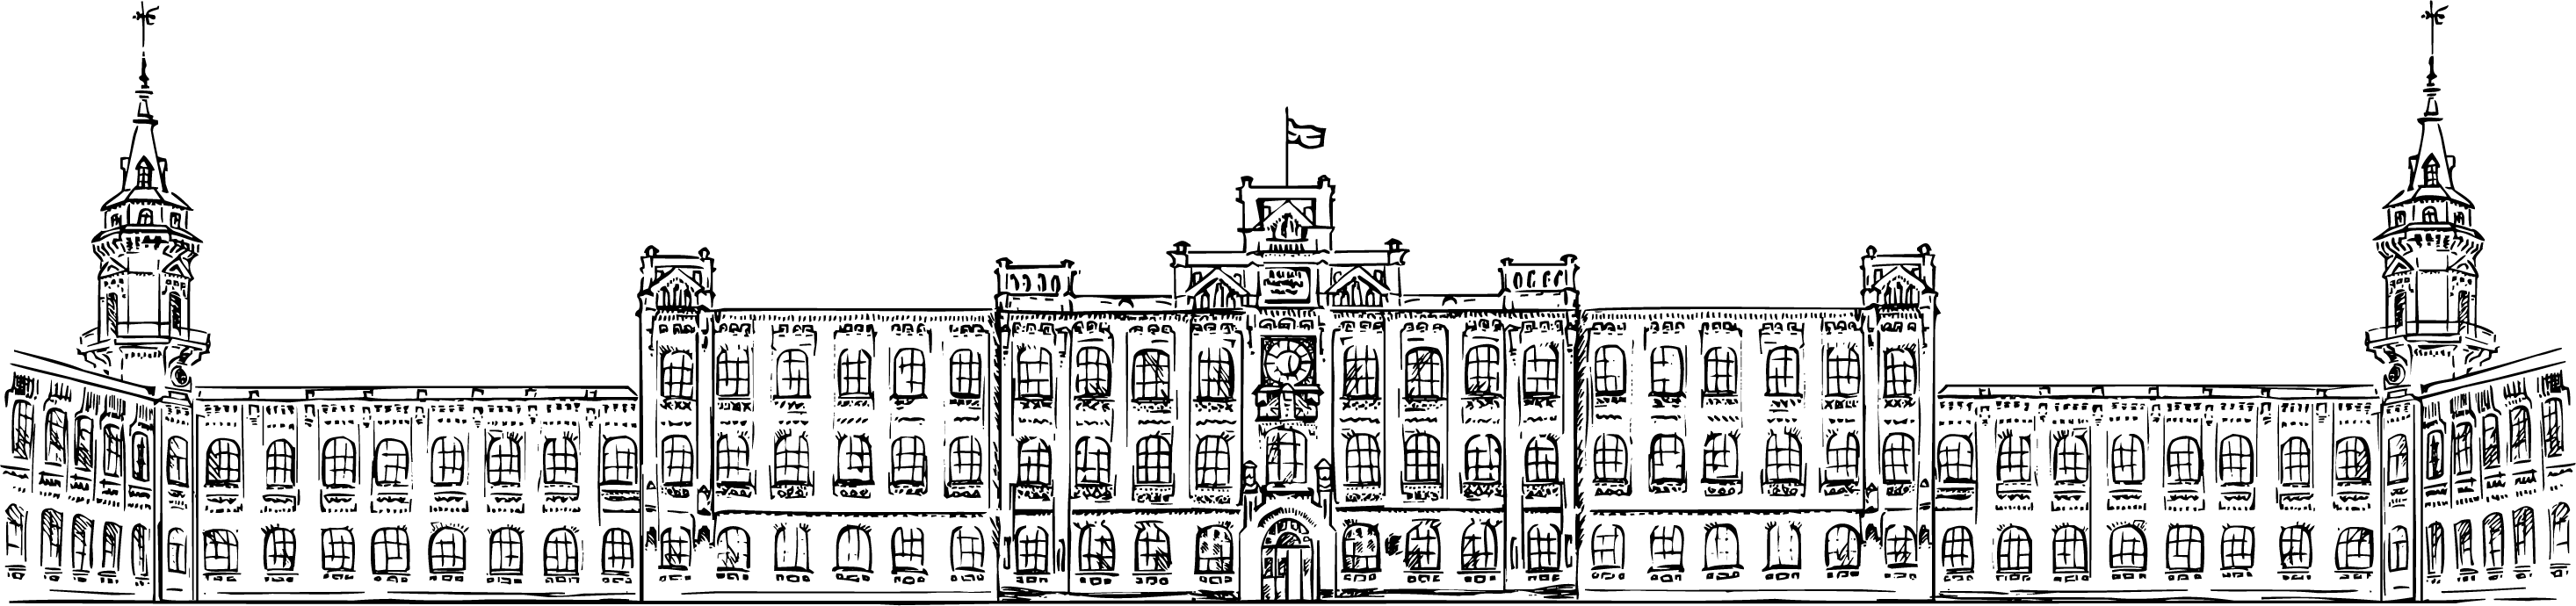
\includegraphics[width=.7\textwidth]{../../../../../../templates/letterhead.png}\end{center}
\begin{center}\large Національний технічний університет України\\«Київський політехнічний інститут імені Ігоря Сікорського»\\[1em]Факультет інформатики та обчислювальної техніки\\Кафедра обчислювальної техніки\end{center}
\vfill\begin{center}\textbf{\LARGE Технології Computer Vision}\\[2em]\textbf{\Large Лабораторна робота №8}\\[.7em]«Технології реконструкції 3D-зображень»\end{center}
\vfill\begin{flushright}\begin{minipage}{.48\textwidth}Виконав: студент 3 курсу ФІОТ,\\групи ІО-41\\\textit{Давидчук А. М.}\\Залікова книжка № 4106\\[1em]Перевірив: \textit{Баран Д. Р.}\end{minipage}\end{flushright}
\vfill\begin{center}Київ --- 2026\end{center}\end{titlepage}
\pagenumbering{arabic}

\section{Тема та мета роботи}
\noindent\textbf{Тема:} технології реконструкції 3D-зображень.

\medskip\noindent\textbf{Мета:} дослідити створення стереопари, стереозіставлення, обчислення диспаритету та відновлення просторових координат.

\section{Завдання роботи}
Розробити Python-скрипт тривимірної реконструкції об'єкта за цифровими зображеннями. Реалізовано віртуальну відкалібровану стереокамеру: дві камери одночасно формують статичні зображення асиметричного об'єкта. За відомими відповідностями обчислюється диспаритет і реконструюється хмара точок. Додано похибку локалізації $0{,}18$ пікселя для перевірки стійкості.

\section{Математична модель}
Для паралельної стереопари з фокусною відстанню $f$ і базисом $B$ координати проєкцій точки мають вигляд
\begin{align}
u_L&=f\frac{X+B/2}{Z}+c_x,&u_R&=f\frac{X-B/2}{Z}+c_x,\\
v_L&=f\frac{Y}{Z}+c_y,&v_R&=f\frac{Y}{Z}+c_y.
\end{align}
Диспаритет $d=u_L-u_R=fB/Z$. Звідси:
\begin{equation}Z=\frac{fB}{d},\qquad X=\frac{(u_L-c_x)Z}{f}-\frac B2,\qquad Y=\frac{(v_L-c_y)Z}{f}.\end{equation}
Якість оцінено евклідовою похибкою $e_i=\lVert p_i-\hat p_i\rVert_2$ та
\begin{equation}\operatorname{RMSE}=\sqrt{\frac1N\sum_{i=1}^{N}e_i^2}.\end{equation}

\section{Архітектура рішення}
\begin{figure}[H]\centering
\begin{tikzpicture}[node distance=.6cm,block/.style={draw,rounded corners,align=center,minimum width=2.75cm,minimum height=.8cm,fill=blue!7},arrow/.style={-{Latex},thick}]
\node[block](a){3D-об'єкт\\4400 точок};\node[block,right=of a](b){Ліва і права\\проєкції};\node[block,right=of b](c){Стереопара};
\node[block,below=of c](d){Диспаритет\\$d=u_L-u_R$};\node[block,left=of d](e){Тріангуляція\\$X,Y,Z$};\node[block,left=of e](f){Хмара точок\\і похибка};
\draw[arrow](a)--(b)--(c)--(d)--(e)--(f);
\end{tikzpicture}\caption{Блок-схема стереореконструкції}
\end{figure}

\section{Результати}
Параметри стереопари: $f=520$ пікселів, $B=0{,}22$ м, розмір кадру $640\times480$. Об'єкт складається з прямокутної основи та пірамідальної верхньої частини.
\begin{figure}[H]\centering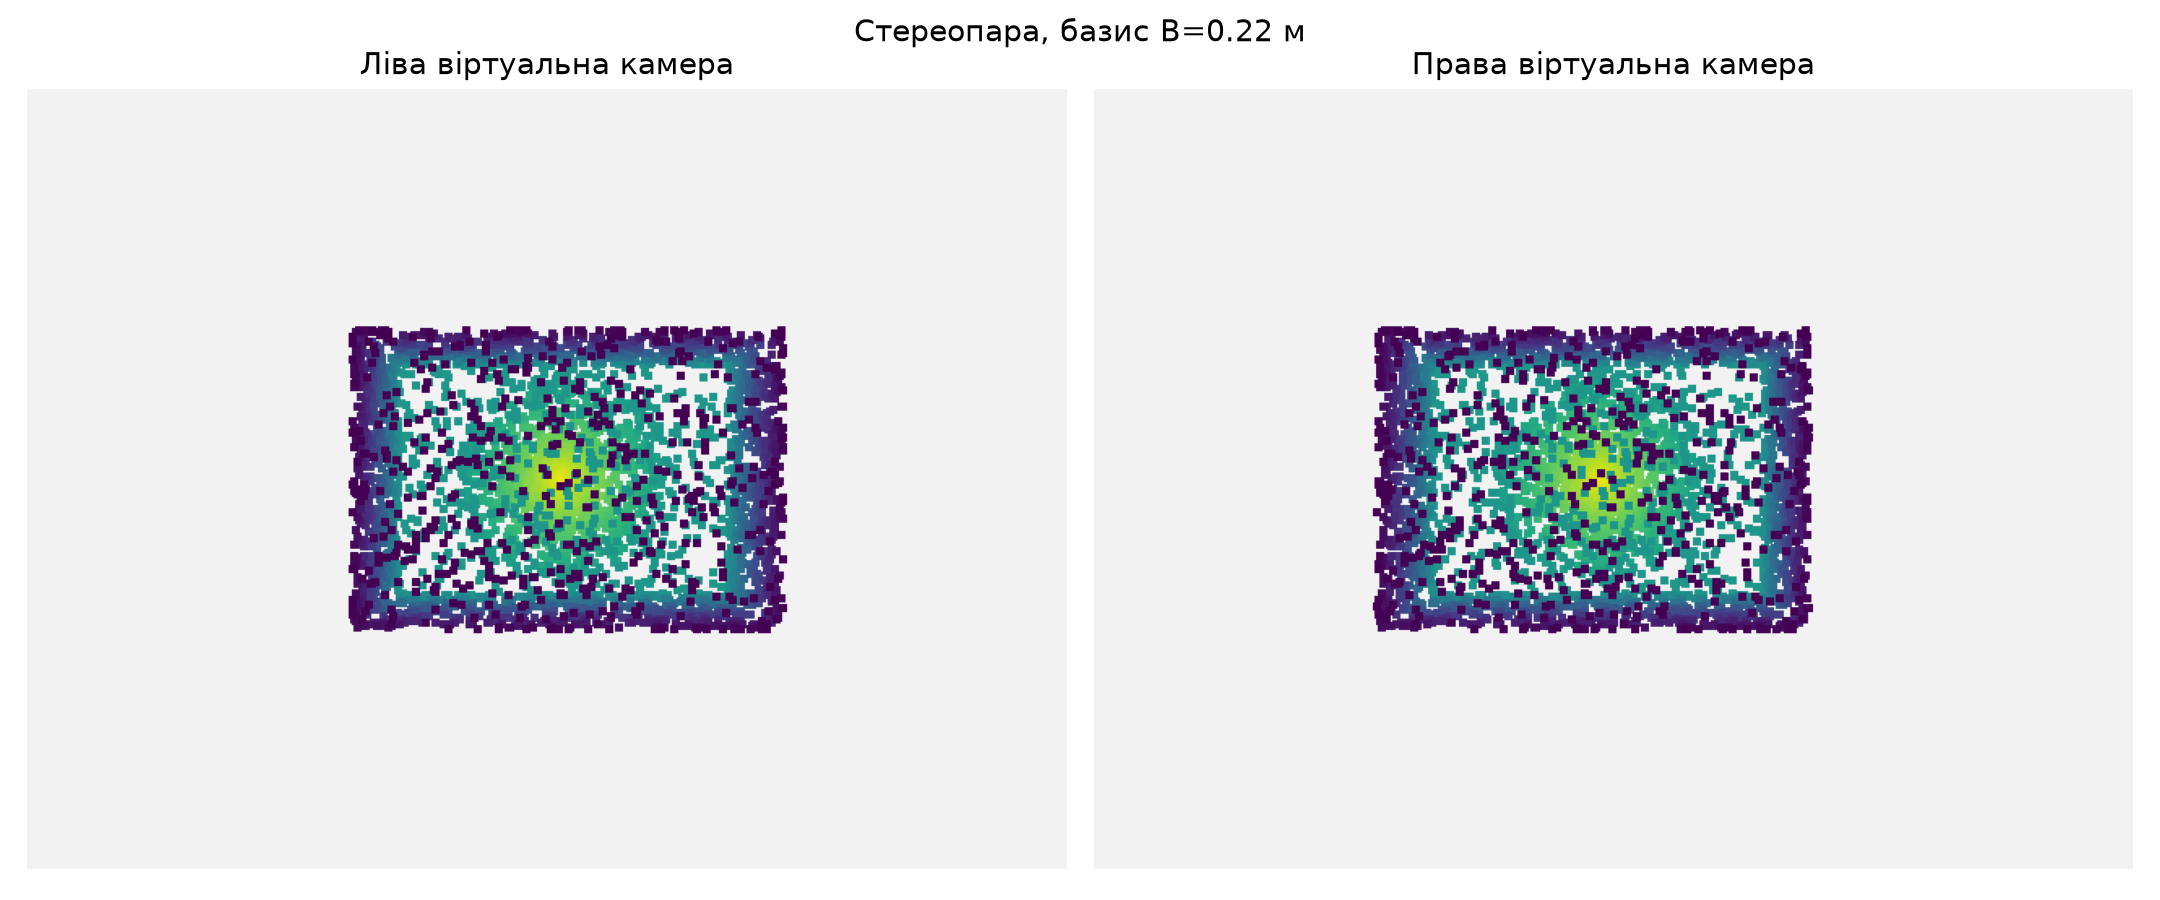
\includegraphics[width=.96\textwidth]{../results/stereo_pair.png}\caption{Синхронна стереопара}\end{figure}
\begin{figure}[H]\centering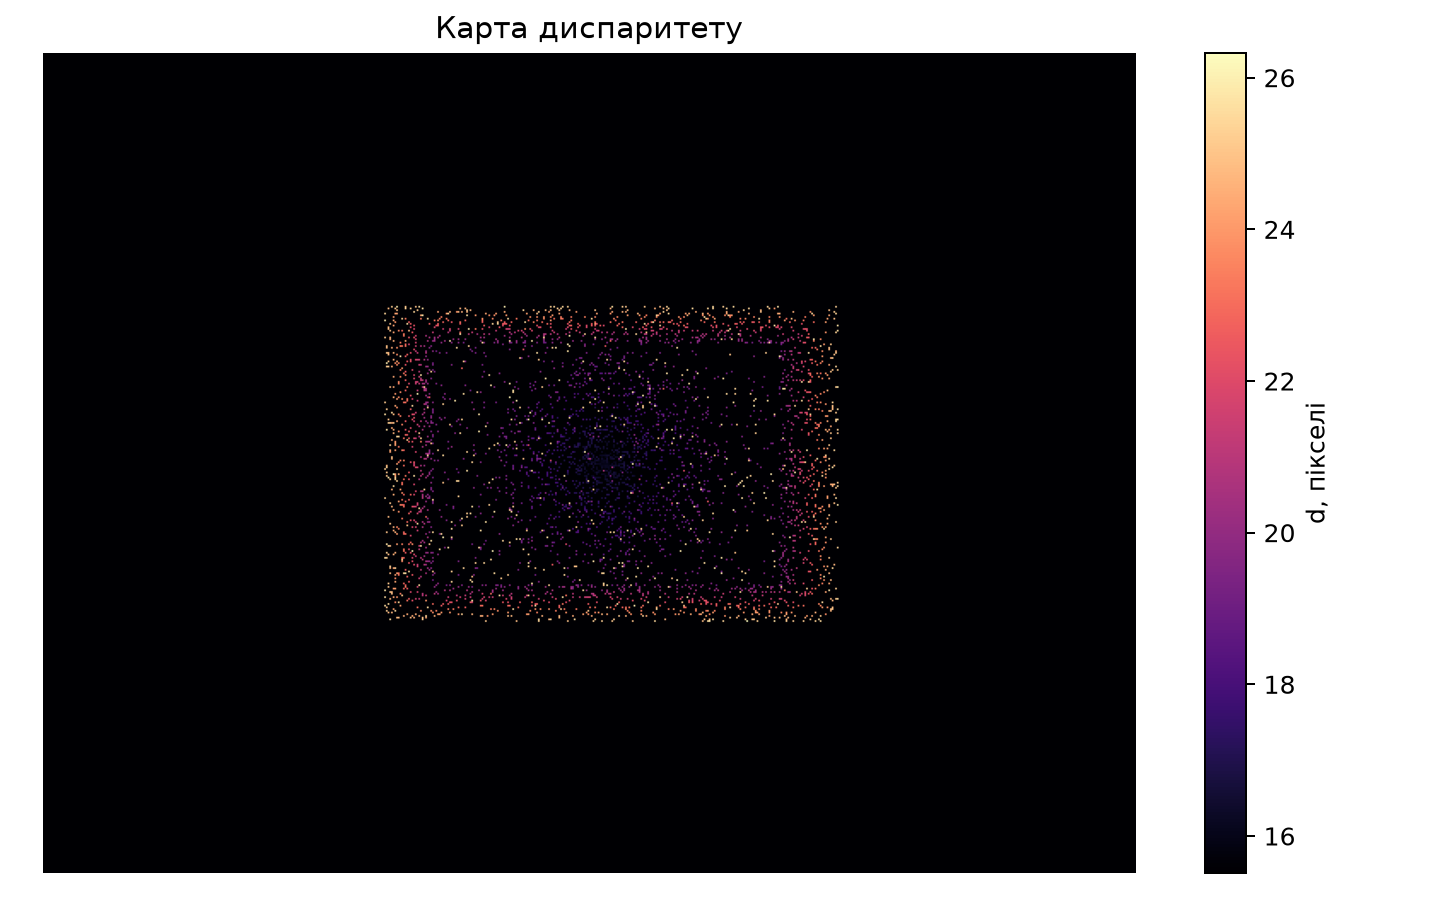
\includegraphics[width=.78\textwidth]{../results/disparity_map.png}\caption{Карта диспаритету}\end{figure}
\begin{figure}[H]\centering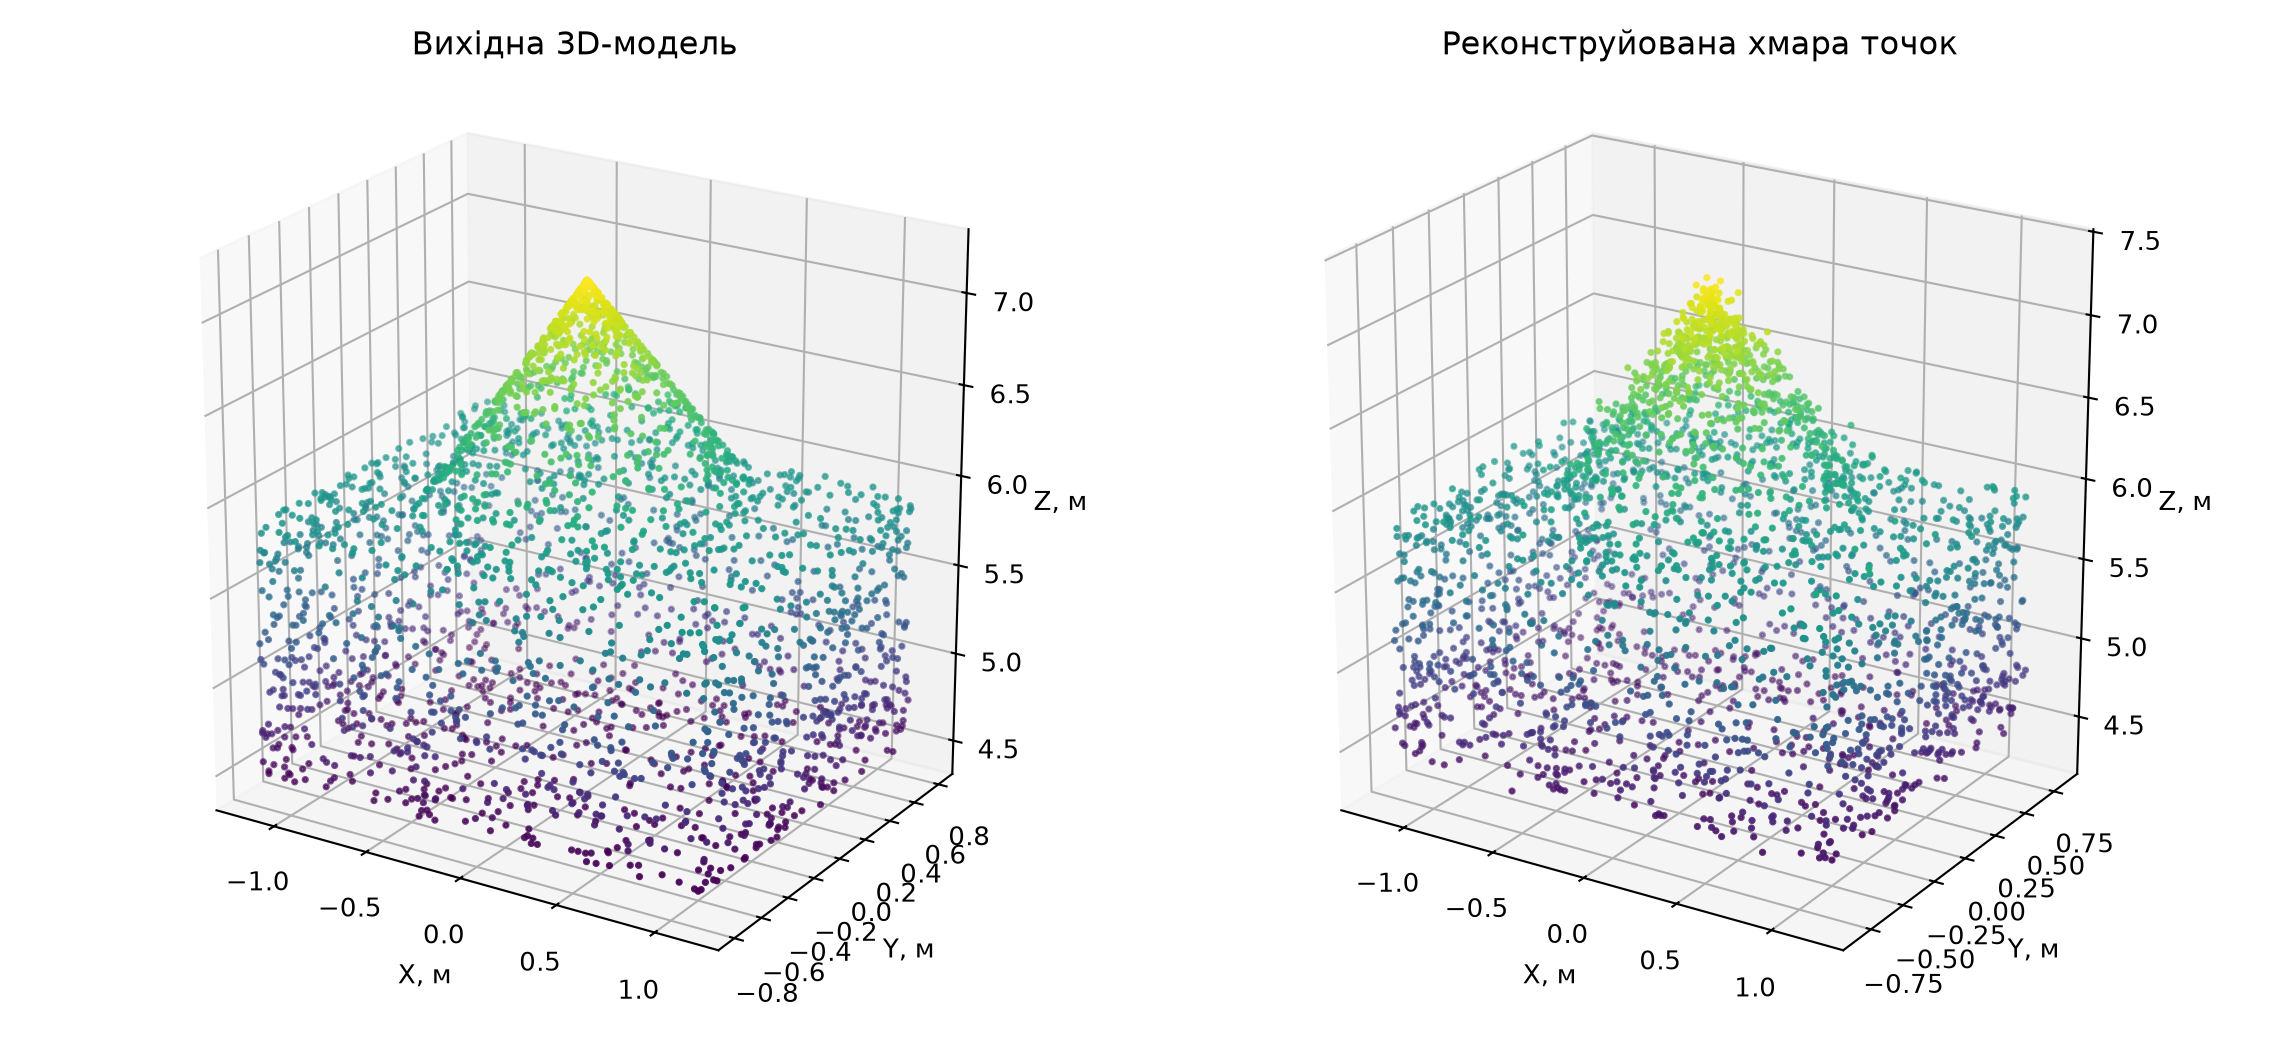
\includegraphics[width=.98\textwidth]{../results/reconstruction.png}\caption{Порівняння вихідної та реконструйованої хмар точок}\end{figure}
\begin{table}[H]\centering\caption{Кількісна оцінка реконструкції}
\begin{tabular}{lr}\toprule Показник&Значення\\\midrule Кількість точок&4400\\Середня похибка&0,057746 м\\RMSE&0,074103 м\\95-й процентиль&0,150162 м\\\bottomrule\end{tabular}
\end{table}
Реконструкція зберігає прямокутну основу та пірамідальну частину. Зростання розкиду по осі $Z$ пояснюється оберненою залежністю глибини від диспаритету: однакова субпіксельна похибка сильніше впливає на дальші точки.

\section{Структура проєкту}
\begin{verbatim}
lab8/
|-- src/main.py
|-- results/stereo_pair.png, disparity_map.png,
|   reconstruction.png, metrics.csv
|-- requirements.txt
`-- docs/main.tex, main.pdf
\end{verbatim}

\section{Висновки}
Реалізовано повний обчислювальний цикл стереореконструкції: формування двох незалежних проєкцій, обчислення диспаритету, тріангуляція та кількісна верифікація. Для 4400 точок середня похибка становить 5,77 см, RMSE --- 7,41 см. Експеримент підтвердив роль фокусної відстані, базису та точності зіставлення у відновленні глибини.

\section{Лістинг програми}
\VerbatimInput[fontsize=\small,numbers=left,breaklines=true,frame=single]{../src/main.py}
\end{document}
